In order to read a barcode, we first have to localize it in a given image. We implemented two approaches. Gradient+Blur is a simple algorithm, with which we had some initial success. We later discarded it in favor of the much more successful Line Segment Detector approach. Both are detailed in this chapter.

\subsection{Gradient+Blur}
Our initial localization attempt showed limited success, but is conceptually very simple. The Gradient+Blur approach seeks to exploit the strong boundaries between the (white) background area and black bars in a standard barcode. In a few words; Detect edges on the image, then blur the result to remove noise and apply a threshold to the result. Open and close the resulting shapes, then select the biggest one. We will now go trough the steps in more detail.

\begin{enumerate}
	\item Edge Detection
	
	We begin by detecting edges with the Sobel operator. We calculate the absolute
  difference of the x- and y-gradients $\abs{\partial_x I - \partial_y I}$,
  discarding direction information.
  This leads to slightly worse results for barcodes rotated by about 45 degrees. The resulting image will usually contain large amounts of noise. This is fixed in the next step. 

	\item Blur+Threshold
	
	Next, we blur the previous result to smooth out the noise and apply a threshold afterwards. The blur is a normalized box filter of size 9. Note that 'noise' here refers not only to image imperfections, but also noise in the absolute gradient which might be a result of complex textures or other sources. The threshold is not set as a constant brightness of 127. Instead, we calculate the mean brightness of the image, add that value to 255 and divide by 2. This simple extra step gives slightly better results when dealing with very noisy images.
	
	\item Close Forms
	
	The next two steps are very similar operations. First we \emph{close} the remaining white areas. This means we first dilate the image, then erode it by the same amount. Dilation creates a new image in which a pixel is set to white if there is at least one white pixel within a given radius white in the original image. More intuitively, white pixels grow outwards. Erosion is the opposite operation; A pixel is set to black, unless all pixels in the radius are white.  This \emph{closes} empty spaces between neighboring and inside of structures, while structures with no neighbors will remain unchanged. At this point, the barcode will ideally have merged into a solid shape, 
	
	\item Open Forms
	
	Opening the forms is similar to closing, but in reverse order; First eroding, then dilating by the same amount. This will eliminate small structures (which is not actually important at this point), while straightening edges on larger structures. 
	
	\item Selection
	
	Finally, we select the largest structure to be the most likely location of the barcode in the original image. In most cases, our result will be a jagged shape, only roughly tracing a rectangle. To simplify matters going forward, we now find the minimal area rectangle around the selected structure. This will get passed into the boundary detection step.
\end{enumerate}

\subsection{LSD}\label{sec:LSD}
This localization method is based on the LineSegmentDetector algorithm
\cite{GromponevonGioi2012}, which is implemented in OpenCV 3 in the
cv::LineSegmentDetector class \cite{Bradski2017}. The algorithm detects line
segments in an image, such as the segments formed by the bars in a barcode.
On a high level, it works by first calculating the image gradient and assigning
to each pixel a unit vector perpendicular to the gradient, resulting in a
\emph{level line field}. Pixels with a gradient magnitude under a certain
tolerance are discarded. Connected pixels with similar level line angles are clustered
together and form a \emph{line support region}. To each line support region, a
rectangle is fit which covers the whole region. To limit the number of false
detections, the rectangle is only accepted as a line segment if the number of
covered pixels with aligned level lines is high enough relative to the total number of
covered pixels. The exact threshold is based on a statistical model (\emph{a
  contrario} method), so that the rectangle is only accepted if,
in a purely random level line field, the found ratio of aligned level lines is unlikely.
Before a rectangle is rejected, some variations of the rectangle's parameters
are tried.

The barcode localization method is taken from \citeauthor{Creusot2016} \cite{Creusot2016} with minor modifications. First we run
the LineSegmentDetector provided by OpenCV on the image. We use default
parameters, except for the first parameter LSD\_REFINE\_NONE, which disables
refinement of line segments. We found that line refinement tends to break up
barcode bars into multiple segments, e.g. if the bars in the image are not quite
straight due to kinks in the material on which the barcode is printed, or if
there are glare spots on the barcode. This is undesirable, since in the
following steps we rely on the length of line segments in the barcode to be similar.

Next we want to find a line segment which belongs to a barcode bar approximately
in the middle of the barcode. To each detected line segment, a score is assigned
based on how many other line segments might belong to bars of the same barcode as the first
one. Two line segments are regarded as possibly belonging to the same barcode, if
\begin{enumerate}
\item their centers are not too far apart,
\item they have similar length,
\item they have similar angles and
\item their projected intersection covers most of the smaller segment.
\end{enumerate}

Calculation of the first three distance measures is straightforward: Let $c_i$
be the center positions, $l_i$ the segment lengths and $\alpha_i$ the segment angles, where the index $i=1,2$
denotes the first or the second line segment, respectively. The used criteria are
\begin{equation*}
d_{\text{center}}\coloneqq\frac{\norm{c_1-c_2}}{l_1}<1,\qquad \frac{\abs{l_1-l_2}}{l_1}<0.3,\qquad \abs{\alpha_1-\alpha_2}<0.1\,.
\end{equation*}
Two lines fulfilling the first three criteria might still not be arranged like
barcode bars, if they are displaced along the line direction. To catch these
cases, we project the second line onto the first and check that the intersection
is large enough relative to the length of the smaller line.

For each line segment which fulfills the criteria, \citeauthor{Creusot2016}
increment the score of the first line segment by one. Instead, we increment the score of the
first line segment by $1-d_{\text{center}}$. This effectively weighs the score by the distance
between the line segments, which favors line segments which lie in
the middle of the barcode.

Finally, we select the line segment with the highest score. This line segment
should correspond to a barcode bar in the middle of the barcode.
\begin{figure}[t]
\center
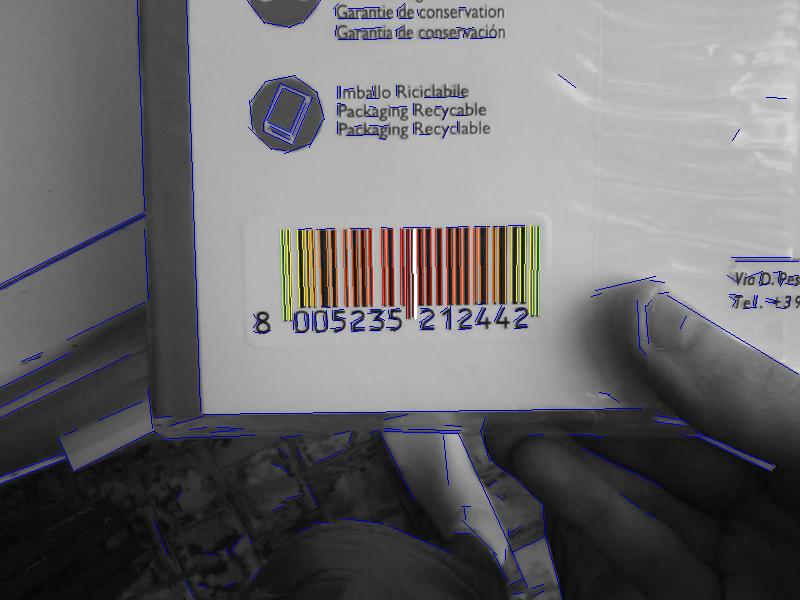
\includegraphics[width=0.6\textwidth,natwidth=800,natheight=600]{img/lsd.jpg}
\caption{LSD localization. The best line with the highest score is drawn in white.}
\label{lsd}
\end{figure}

%%% Local Variables:
%%% mode: latex
%%% TeX-master: "00Ausarbeitung.tex"
%%% End: